\chapter{Conclusions}

\begin{changemargin}{1.0cm}{1.0cm}
\abstractpreamble{It is known that Cr provides protection to stainless steel through a passive protective layer, but this becomes ineffective to protect the steel under irradiation as Cr is depleted from the grain boundary.  \Acrlong{pgm}s also provide a mechanism to protect steel from corrosion, and experimentation or simulations may be used to investigate whether they can maintain high enough concentrations at the surface to continue to protect the steel against corrosion under irradiation.  If either of the two chosen \acrshort{pgm}s, Pd or Ru, are depleted at the grain boundary under irradiation as well as depletion of Cr, the steel will become susceptible to corrosion.  \\
\\
Experimental testing is cheaper, more controllable and more rapid at causing damage in a targeted volume if an ion beam is used rather than a neutron source.  Either source will cause the target material to become radioactive.  It is important to be able to calculate how radioactive, and how long after irradiation (to the desired damage, in DPA) it will be until the material is safe to be handled.\\
\\
Computer simulations to simulate radiation damage will be much too large and complex for first-principles calculations.  Damage cascades require thousands of atoms and typical damage rates take years to reach in practice.  Simulations will need to use either classical molecular dynamics or kinetic monte carlo to encapsulate the much larger volumes of atoms, to contain the atoms effected by the damage cascade, and to represent the grain boundary.  This requires the derivation of an appropriate interatomic potential using experimental data and first-principles data where it is not available, or where it is either impossible or impractical to measure.}
\end{changemargin}






\section{Inter Granular Stress Corrosion Cracking}

Austenitic stainless steel is particularly susceptible to inter granular stress corrosion cracking.  It has good properties, including a good resistance to corrosion due to its high Cr and Ni content.  Under irradiation, the Cr at grain boundaries is depleted with the formation of Cr carbides.  Three requirements for inter granular stress corrosion cracking to occur are:

\begin{itemize}
\item a susceptible material (austenitic stainless steel)
\item stress, welds, swelling, pressure, any applied stress (high pressure in reactor environment, swelling due to irradiation)
\item a corrosive environment (radiolysis of water)
\end{itemize}

The passive Cr layer, under normal conditions, protects the steel from corrosion.  The steel is made up from small grains, and the surface of these grains of crystalline metal are where the protective layer covers.  During irradiation, Cr is depleted, forming Cr carbides between the grain boundaries.  As the percentage of Cr drops, the surface becomes prone to corrosion.

Small quantities of platinum group metals may be added to a steel to also increase the corrosion resistance of the steel.  Platinum group metals are rare and much more costly that Fe, Ni, Cr.  Where irradiation is not present, it has been shown experimentally that the benefit due to Pd is lost due to the formation of Pd-Mn nanoparticles, where Mn is present in the steel, although no such particles are present when Pd was replaced by Ru.  Pd does provide corrosion protection via cathodic modification when Mn is reduced to very small amounts as it no longer forms Pd-Mn precipitates during sensitisation.  The outstanding question is whether or not Pd or Ru are depleted, enriched or are unaffected at the grain boundary when under irradiation.



%%%%%%%%%%%%%%%%%%%%%%%%%%%%%%
% Activity
%%%%%%%%%%%%%%%%%%%%%%%%%%%%%%

\section{Predicting Ion Induced Radioactivity}

Testing a material inside a nuclear reactor is an expensive experiment.  There are many more ion sources around the world than high flux neutron sources, and ion beams are easier to direct due to the charge of the ion versus the neutral charge of the neutron.  The ion energies required to create similar sized damage cascades in the material are high enough to also have a chance of transmuting the target nuclei.  These transmuted nuclei are most likely going to be radioactive.  To reach damage dose levels comparable to a component in a \acrshort{gen4} reactor by the end of its life (up to 200 \acrshort{dpa}), the target material will become dangerously radioactive. 

Bateman's equation may be used to calculate the amount of an isotope in a decay chain of several isotopes, and thus how radioactive an isotope would be after a certain time.  Major modifications were required to be made to the equation to also include branching factors and source rates for isotopes generated by an ion beam.

\subsection{Modified Equation}

Whilst the equation was first tackled by solving the differential equations head on, it became obvious that using Laplace transforms would be the logical choice; this was also the route Bateman followed when deriving the original equations.  Once transformed, a numerical algorithm (Gaver-Stehfest) was programmed and used to solve, with some success.  

The numeric method is not an exact solution, and the errors incurred often resulted in negative amounts of an isotope, and this was unacceptable.  More progress was made towards solving the problem analytically, and by using partial fractions, obviating the need for a numerical method. 

The analytic solution was tested against a simple numeric solver and the results were in good agreement between the modified equation and numeric solutions (appendix \ref{section:decaypo216numeric}).

\subsection{Activity Code}

The Activity code was created to automate the process of calculating the activity of an ion irradiated target.  The program:

\begin{itemize}
\item reads in simulation details (target composition, thickness, duration etc)
\item reads in ion cross section data from the \acrshort{tendl} database
\item processes \acrshort{srim} exyz data points
\item calculates the amount of each isotope by the end of the simulation
\item calculates the activity of each isotope and the dose that an average human would be exposed to
\end{itemize}

A number of simplifications are made to the model but it predicted the radioactivity of certain peaks reasonably well with a sample of proton irradiated pure Fe.  Given more time a range of alloys would also be irradiated by a proton beam and, once their activity is measured at several time intervals after irradiation, they would compared to the activity predicted by the Activity code.

The first version of the Activity code was replaced by a second version that used Python rather than Fortran.  The first version was more cumbersome for new users and it crashed for certain isotope, and these problems were fixed in the new version.



\subsection{Iron Irradiation}

During the experimental stage of this work it was determined that the isotope to focus on would be Cobalt-55 and the associated 931keV peak it generates would be the peak to measure.  The equipment was calibrated specifically for the purpose of measuring this gamma.  If this is the case then the value predicted by the Activity V2 computer code is in good agreement (table \ref{table:activityResultsCompared}). 

However, the second version of the Activity code collates and displays data more clearly than the first version.  It is clear that there should also be a nearby 935KeV gamma from the decay of Manganese-52.  The sum of these nearby gammas is predicted to be almost 120kBq and, if both peaks were tallied in the experimental work due to the energy resolution of the detector, the predicted value is three times that of the measured value of 44kBq.

It is quite possible that the code is giving a value three times larger than expected and reasons for this will be discussed below.


\subsection{Molybdenum Irradiation}

Similar to the results discussed for Iron, the activity results computed for Molybdenum have positive and negative attributes.  There are gaps in the available cross section data, but the most prominent gammas are predicted by the computer code.  The radioactivity computed is too high, but for each of the five peaks measured by experiment, the values are out by a similar factor.


\subsection{Beam Flux Reduction and Gamma Attenuation}

The cross section data used in the second version has been checked for a number of cases against EXFOR data and is in good agreement with this.  Certain data for reactions is missing in particular those of observationally stable and isotopes with extremely long isotopes.

Thin foils are ideal to compare experimental results to the data files and activity code as ions will not lose a great deal of energy travelling though such a shallow target.  However, the much thicker targets used here for Iron and Molybdenum reduce ion energies significantly if not completely.

It could be argued that as ions pass through the target the energy and intensity of the beam decreases, and this is not modelled with the activity code.  By imagining the target as thin laminae perpendicular to the beam it is easy to consider that the ions will enter the first layer and lose those that react with target atoms.  As the beam enters the next lamina it will have a lower energy and a lower intensity.

The change in energy is accounted for by virtue of the \acrshort{srim} exyz ion trajectory file but how the beam intensity decreases is not.  How many ions are captured through nuclear reactions and is it a significant percentage of the total number of ions?  Particles and residuals were calculated to be produced at a rate of approximately $6\times10^{10}$ per second for the Iron target and $7\times10^{10}$ per second for the thick Molybdenum target.  The beam rates were $3 \times 10^{12}$ and $3 \times 10^{13}$ protons per second respectively and so, even if the estimate that a proton was removed for each reaction the beams would only lose 2\% and 0.3\% of their intensity due to transmutation reactions.

Another possibility for the over estimate in prediction is the attenuation of gammas travelling through the target material to the detector.  This was discussed in the work of my colleague\cite{johnhewett} and the inhomogeneous distribution of radioactive material in the Molybdenum target was discussed in this work (section \ref{section:estimatingmoactivity}).  Calculations using the \acrshort{nist} attenuation coefficient for Molybdenum show that 500keV gammas have their intensity reduced to 91\% through a 1.0cm target.  The intensity of 1MeV gammas is reduced to just 94\% through the same target.

The reduction through loss of ions due to reactions and attenuation of gammas does not explain the increase in predicted activity.  There may be another reason behind this, or there may be issues with the experimental work.


\subsection{More Experimental Data Required}

I have not had a great deal of experience practically measuring gammas, and I would expect there to be errors introduced due to my own inexperience.  The range of beam energies, elements and beam duration are also very restricted.

In past experimental work discussed in section \ref{section:exfordata}, thin foils were used to measure reaction probabilities, and this data influences models such as TALYS.  In some two out of the three examples reviewed, the data beam energy was degraded using a stack of foils perpendicular to the beam, with those closest to the aperture receiving the highest energy protons.  It is hard to imagine whether foils stacked in this way would be much different to a solid target of the same thickness, but this should be tested experimentally.

Ideally a range of target materials of varying thicknesses would be irradiated with protons of energies ranging up to the limit of the cyclotron, perhaps 60MeV, and the Gamma spectra of each measured at set times after irradiation.  This data would be compared to the gamma lines predicted by the activity code to help give a better understanding of the accuracy of the code.







\subsection{100DPA Activity Predictions}

Using dose rates calculated with \acrshort{srim}, the code was used to predict how radioactive Fe would become at a dose rate of 100DPA.  It assumes the beam source is the Scanditronix MC40 using protons at maximum current for an uninterrupted duration of 134-391 days.  In the worst case scenario, 25MeV protons result in over 20 grays per hour if irradiated to the required damage dose.  However, by reducing the beam energy to 15MeV radioactivity of the target is reduced by a factor of 1,000.  It may be reduced further by lowering the energy to 5 or 10MeV, but for a 0.5mm piece of steel, the ions would not have enough energy to pass through and the damage would be disproportionately concentrated in the top 100-250 microns.

\subsection{Original Contribution}

The modified Bateman equation as derived is an original contribution to knowledge.  The activity code is also an original contribution, and its use shows how adjusting beam parameters will reduce the amount of radioactive material created and the risk to those handling irradiated samples.



\section{Iron-Palladium Potential}

\subsection{Restricting the Potential to Iron-Palladium}

It would be too complex a task to develop an interatomic potential that includes Fe, Pd, Cr, Ni and any other elements that make up a typical sample of austenitic stainless steel; Fe and Pd are the starting point, with the possibility of adding more elements to the potential in the future.

Pd exists in the \acrshort{fcc} state at normal conditions, but Fe is \acrshort{bcc}.  The relatively high percentage of Ni in the steel stabilises the austenitic \acrshort{fcc} structure.  The bulk properties, such as the lattice parameter, bulk modulus, elastic constants and so forth, are experimentally known for Pd.  As Fe doesn't exist in the gamma phase at normal conditions, \acrshort{dft} calculations were used to find the bulk properties of gamma Fe.

\subsection{Collinear Spin \acrshort{dft}}

With most models, there will be a trade off between simplicity, accuracy and the computational cost of the model.  The parameters that had the largest impact on how long a \acrshort{dft} calculation will take to compute are the planewave energy cutoff and number of k-points used to integrate the Brillouin zone.  These should be reduced as much as possible, while keeping the energy and force results within a tolerance determined by the user.

A choice in the complexity of the calculation also had to be decided upon, and this was whether to use a non-spin, collinear spin or non-colinear spin calculation.  Pure Fe under normal conditions has a \acrshort{bcc} structure and energetically favours a ferromagnetic configuration.  Cr also has a \acrshort{bcc} structure under normal conditions, but it's optimum structure magnetically is antiferromagnetic.  Gamma phase Fe (\acrshort{fcc}) is also antiferromagnetic, and so it will be important to include magnetism in the \acrshort{dft} calculations.

The options in increasing complexity, and computational time, are:

\begin{itemize}
\item non-magnetic
\item collinear - suitable for high symmetry, ferromagnetic/antiferromagnetic
\item non-collinear - spin may not be aligned in the same direction
\end{itemize}

For the Fe and Pd calculations, collinear spin was used and the starting configurations of the atoms were set up in accordance with the known configurations i.e. \acrshort{bcc} Fe was configured such that the spins were aligned in the same direction, and \acrshort{fcc} were set up in an antiferromagnetic setting.  The collinear \acrshort{dft} calculations showed that Fe \acrshort{fcc}, where magnetism is taken into account, is slightly tetragonal with the atoms arranged in a \acrshort{fct} structure.

A Python (QECONVERGE) code was developed to automatically converge the aformentioned parameters.  Whilst automation worked well for the planewave cutoff parameters the choice of smearing type, the amount of smearing and number k-points was more difficult to automate.  It was more useful to select a range of k-point values and smearing values and produce 2D force and energy plots so the user could make a decision based on these and choose the parameters that best suit their requirements.

During testing, a much larger number of k-points were needed for the predicted properties of Aluminium to replicate the known properties reasonably well.  Unfortunately, the number of k-points used for Fe and Pd was constrained by the amount of time and the RAM available on the compute nodes.  Ideally, more k-points would have been used, but this was not possible.



\subsection{Bulk Properties of Orthorhombic \acrshort{fcc} Iron}

As pure Fe does not exist in its gamma phase at room temperature, \acrshort{dft} calculations were used in place of experimental data.  As eluded to in the previous section, collinear spin \acrshort{dft} was selected.  Although a smaller number of k-points were used, the calculation lasted for approximately 30 days from start to end.

Rather that calculate the input files manually, a program was created to automate this process (QE\_EOS).  It was designed to cache input and output files for the \acrshort{dft} program, PWscf, such that it would load an output file from the cache if it had already successfully run, to reduce the calculation time.

The relaxed (energy minimised) shape of the antiferromagnetic \acrshort{fcc} Fe was not cubic, but orthorhombic.  The equation of state calculation is specifically for a cubic crystal, but the elastic constants were calculated for the orthorhombic crystal.  From the 9 calculated elastic constants the melting point, bulk modulus, shear modulus and Young's modulus were calculated (section \ref{section:fccferesults} and appendix \ref{section:fefccappendix}).  The resulting structure was stable and were well within a magnitude of the known values for \acrshort{bcc} Fe.  These data are an original contribution to science.



\subsection{Palladium-Iron Configurations as Fitting Data}

To be able to fit the Fe-Pd potentials, the bulk properties of both pure \acrshort{fcc} Fe and \acrshort{fcc} Pd were either calculated or taken from experimental values.  The potentials were then trained to fit this data.  As well as this, a number of configurations of Fe, Pd and Fe-Pd were generated with their atoms slightly displaced from their lattice positions.  This would gave a wider range of atom separations and force values for the fitting program to use.

The force data were entirely from first-principles calculations, and ideally there would have been more configurations and computed with a higher number of k-points.  In addition, a wider range of vacancies, interstitials and mixing concentrations would have been desirable. The atomic percentage on Pd or Ru doped is half a percent which would be better represented with a one \acrshort{pgm} atom in a 4x4x4 \acrshort{fcc} 256 atom supercell rather than the 32 atom cells used, but again this was a constraint imposed by computational resources.



\subsection{Iron-Palladium Potential}

The first derived Fe-Pd potential reproduces the properties of the material with a minimum error of 0.0\% for the cohesive energy for both Fe and Pd, and a maximum error of 8\% for the bulk modulus of Fe.

The cohesive energy and surface energy plots have a number of irregular bumps (fig \ref{fig:v1plots}), and it is hard to say whether or not these are correct without also computing them using \acrshort{dft}.

\begin{figure}[ht] 
  \centering
  \begin{minipage}[b]{0.4\linewidth}
    \centering
    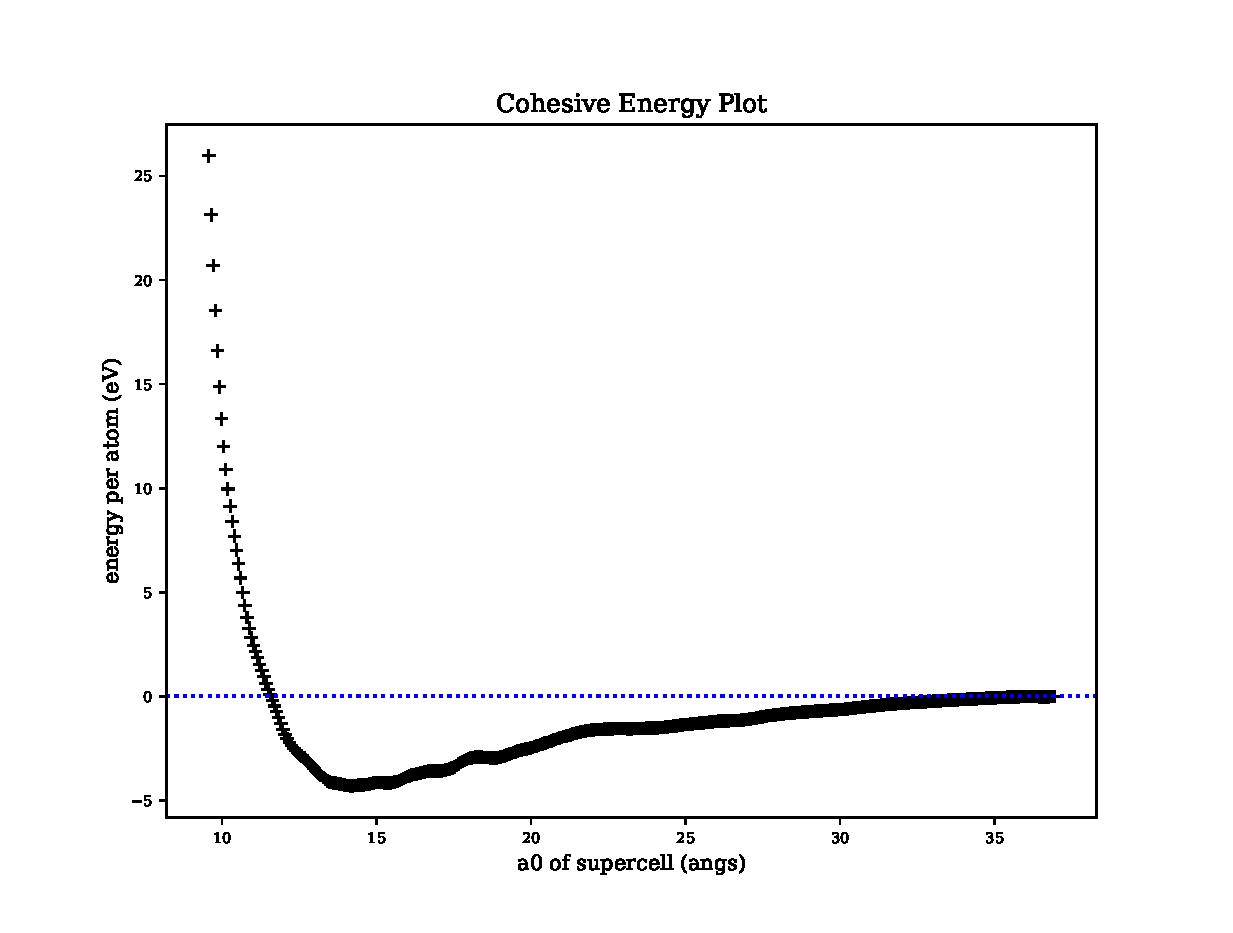
\includegraphics[width=.98\linewidth]{chapters/potentials_fe_pd_ru/pot_fepd_fcc_1/fe_cohesive_energy.eps} 
  \end{minipage}%%
  \begin{minipage}[b]{0.4\linewidth}
    \centering
    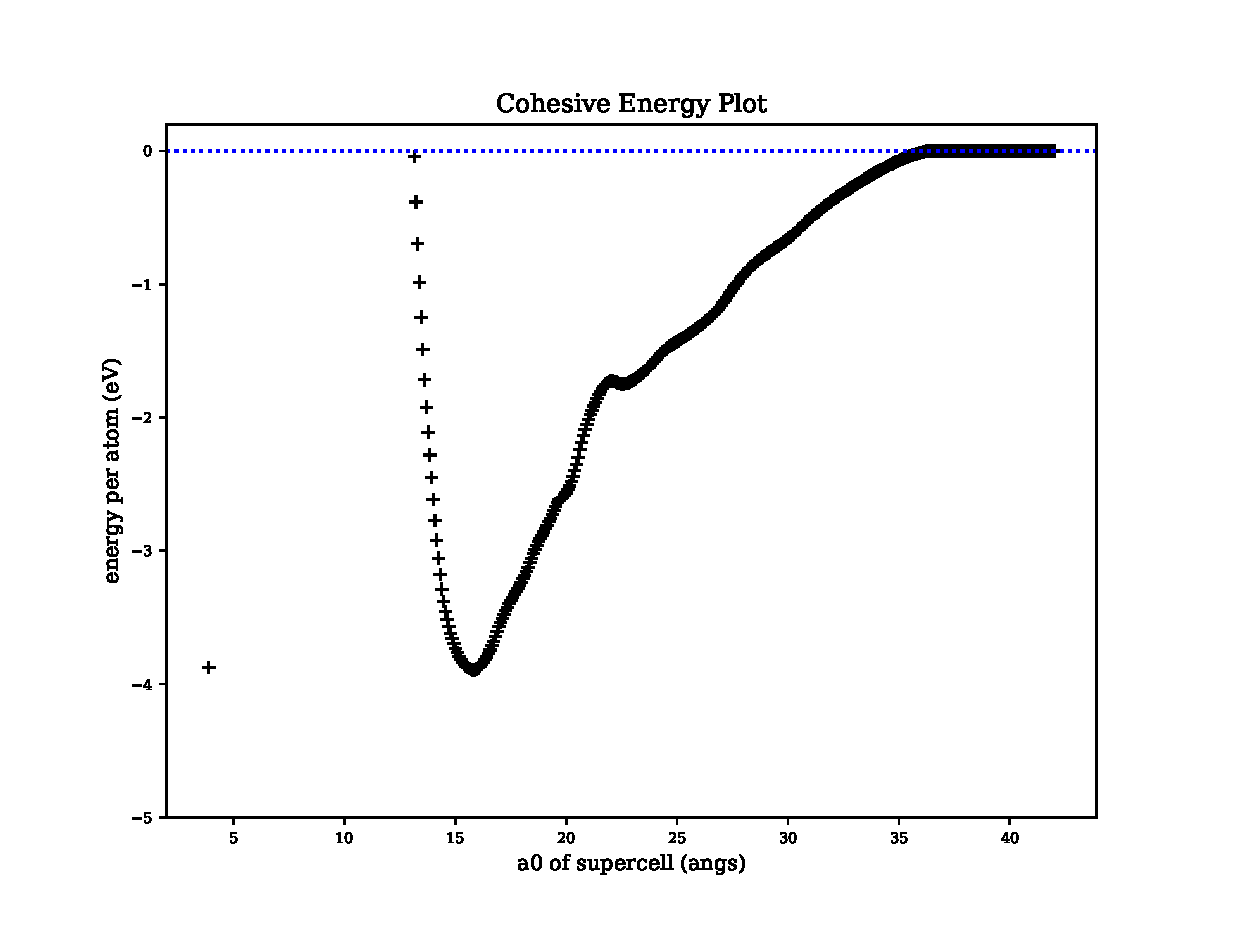
\includegraphics[width=.98\linewidth]{chapters/potentials_fe_pd_ru/pot_fepd_fcc_1/pd_cohesive_energy_zoom.eps} 
  \end{minipage}%%

  \centering
  \begin{minipage}[b]{0.4\linewidth}
    \centering
    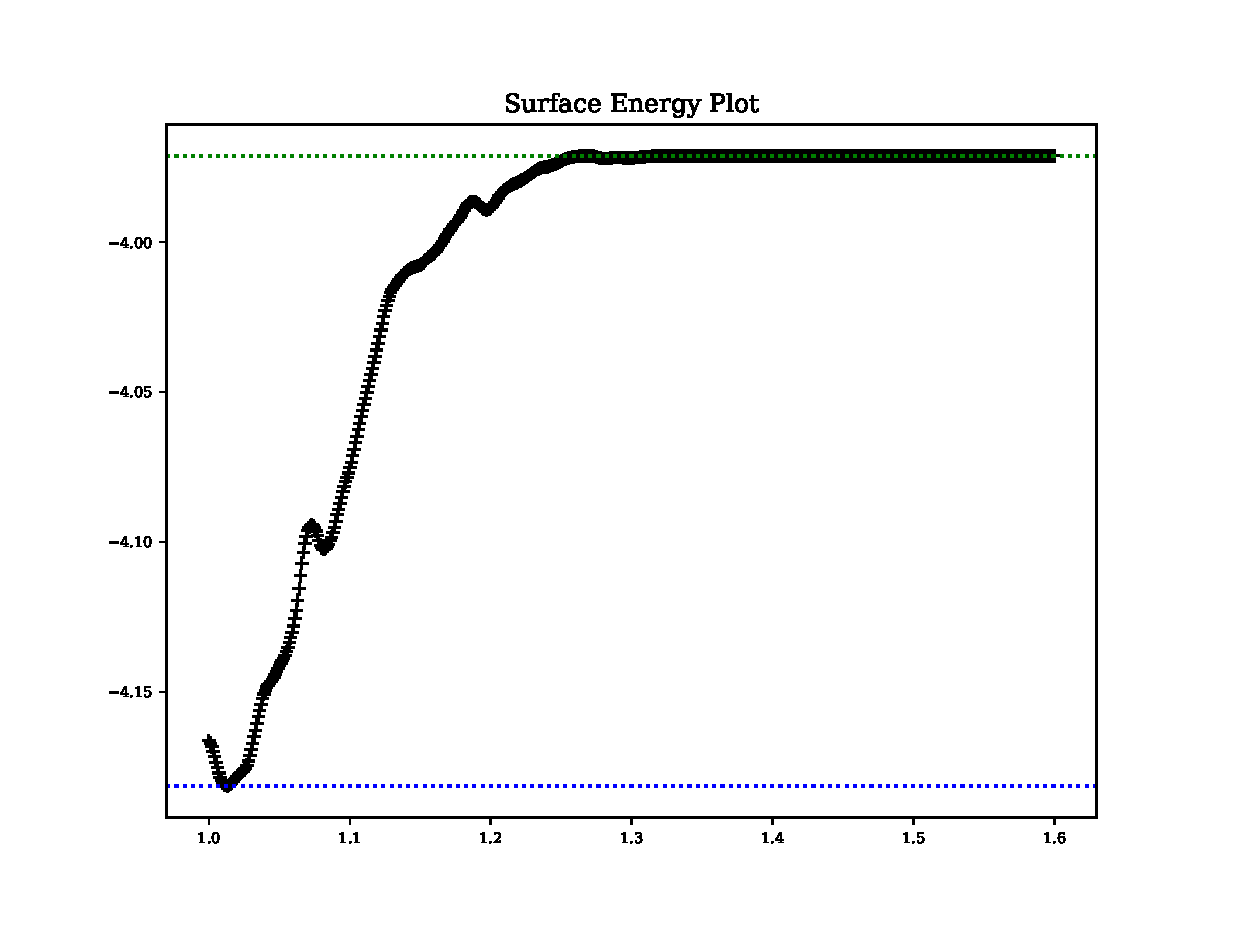
\includegraphics[width=.98\linewidth]{chapters/potentials_fe_pd_ru/pot_fepd_fcc_1/fe_surface_energy.eps} 
  \end{minipage}%%
  \begin{minipage}[b]{0.4\linewidth}
    \centering
    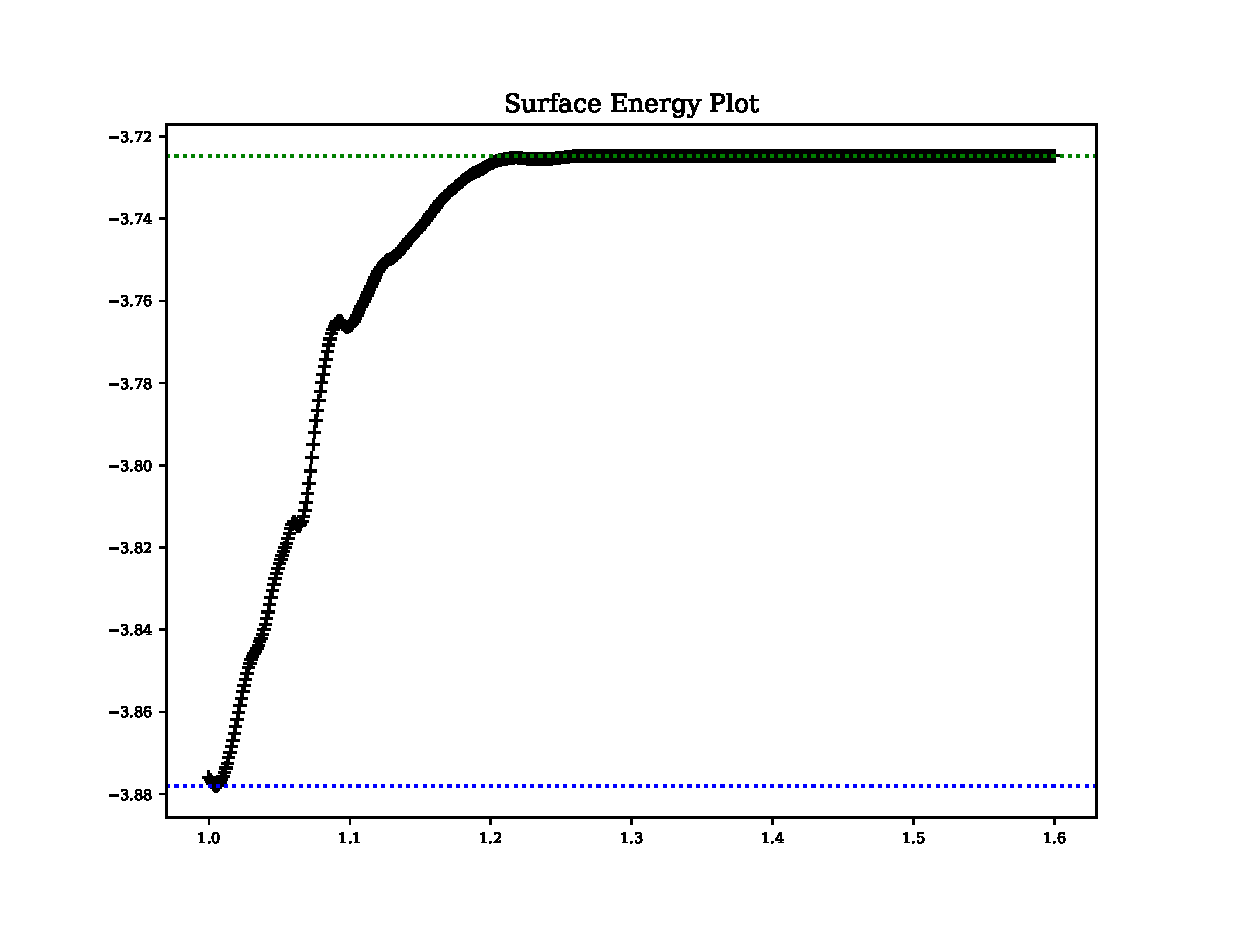
\includegraphics[width=.98\linewidth]{chapters/potentials_fe_pd_ru/pot_fepd_fcc_1/pd_surface_energy.eps} 
  \end{minipage}%%
	\caption{Cohesive energy and surface energy plots - detailed plots in the appendix \ref{fepdv1coh} and \ref{fepdv1se}}  
\label{fig:v1plots}
\end{figure}
\FloatBarrier

The second derived Fe-Pd potential reproduces the properties of the material with a minimum error of 0.0\% for the cohesive energy of Pd and the $C_{22}$ elastic constant for Fe, and a maximum error of 4.8\% for the bulk modulus of Fe.

Despite having a better fit to the properties of the material used, the cohesive energy and surface energy plots are less well behaved than those in the first version (fig. \ref{fig:v2plots}).  The optimisation algorithms blindly fit potentials to the data available, and it is apparent that more \acrshort{dft} computed energies are required for a variety of configurations, including splitting the bulk into two surfaces and expanding atoms from bulk into isolated atoms.

\begin{figure}[ht] 
  \centering
  \begin{minipage}[b]{0.4\linewidth}
    \centering
    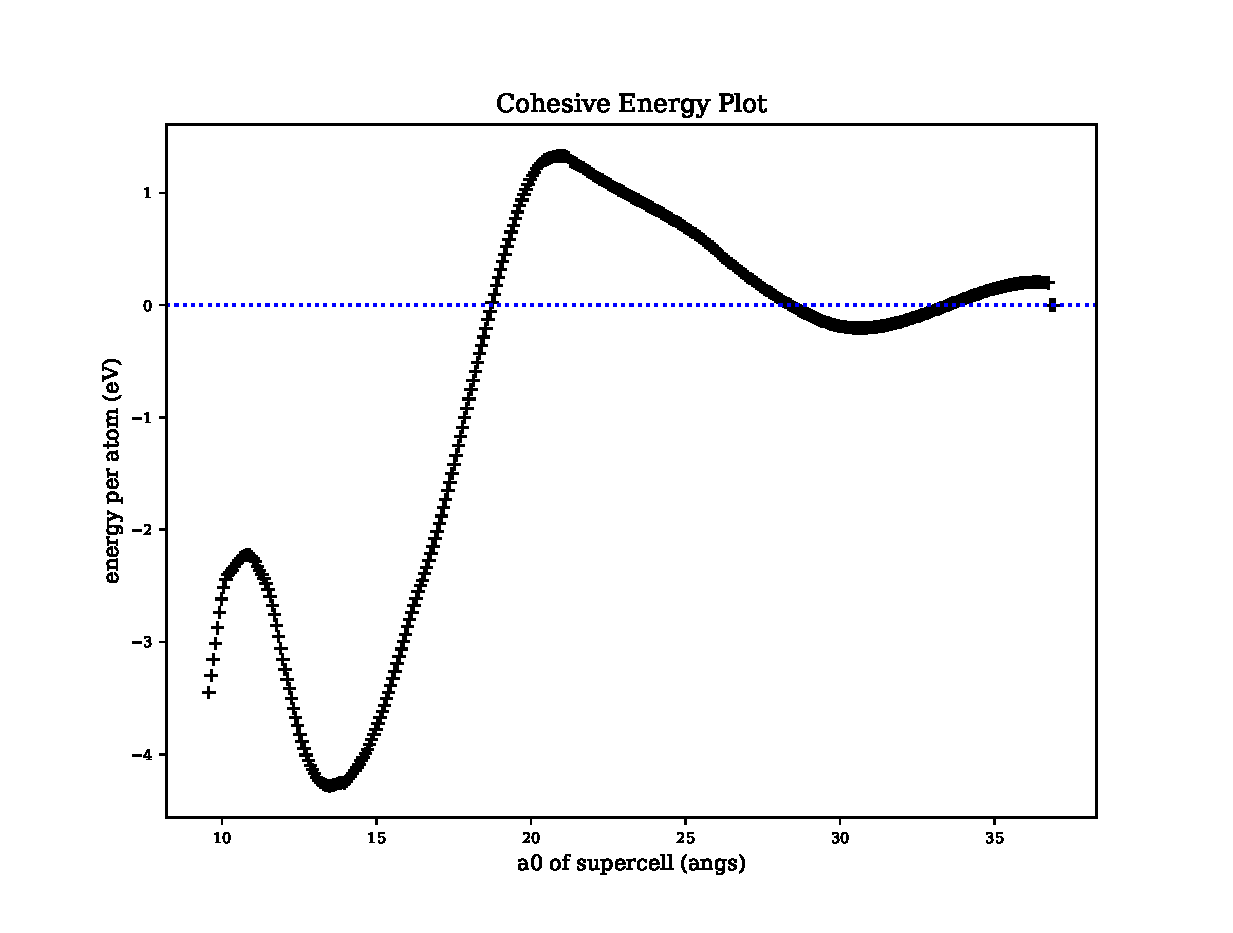
\includegraphics[width=.98\linewidth]{chapters/potentials_fe_pd_ru/pot_fepd_fcc_2/fe_cohesive_energy.eps} 
  \end{minipage}%%
  \begin{minipage}[b]{0.4\linewidth}
    \centering
    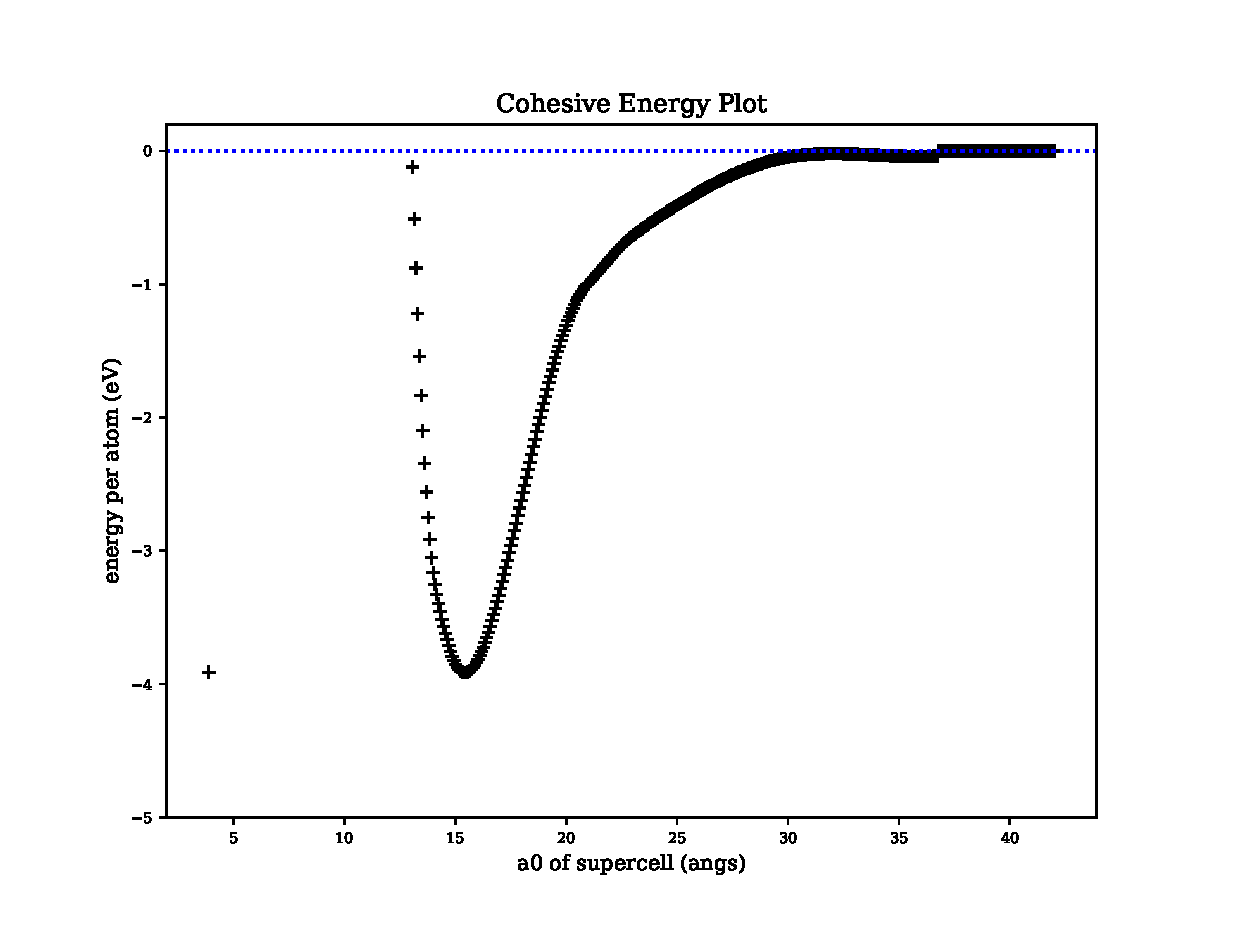
\includegraphics[width=.98\linewidth]{chapters/potentials_fe_pd_ru/pot_fepd_fcc_2/pd_cohesive_energy_zoom.eps} 
  \end{minipage}%%

  \centering
  \begin{minipage}[b]{0.4\linewidth}
    \centering
    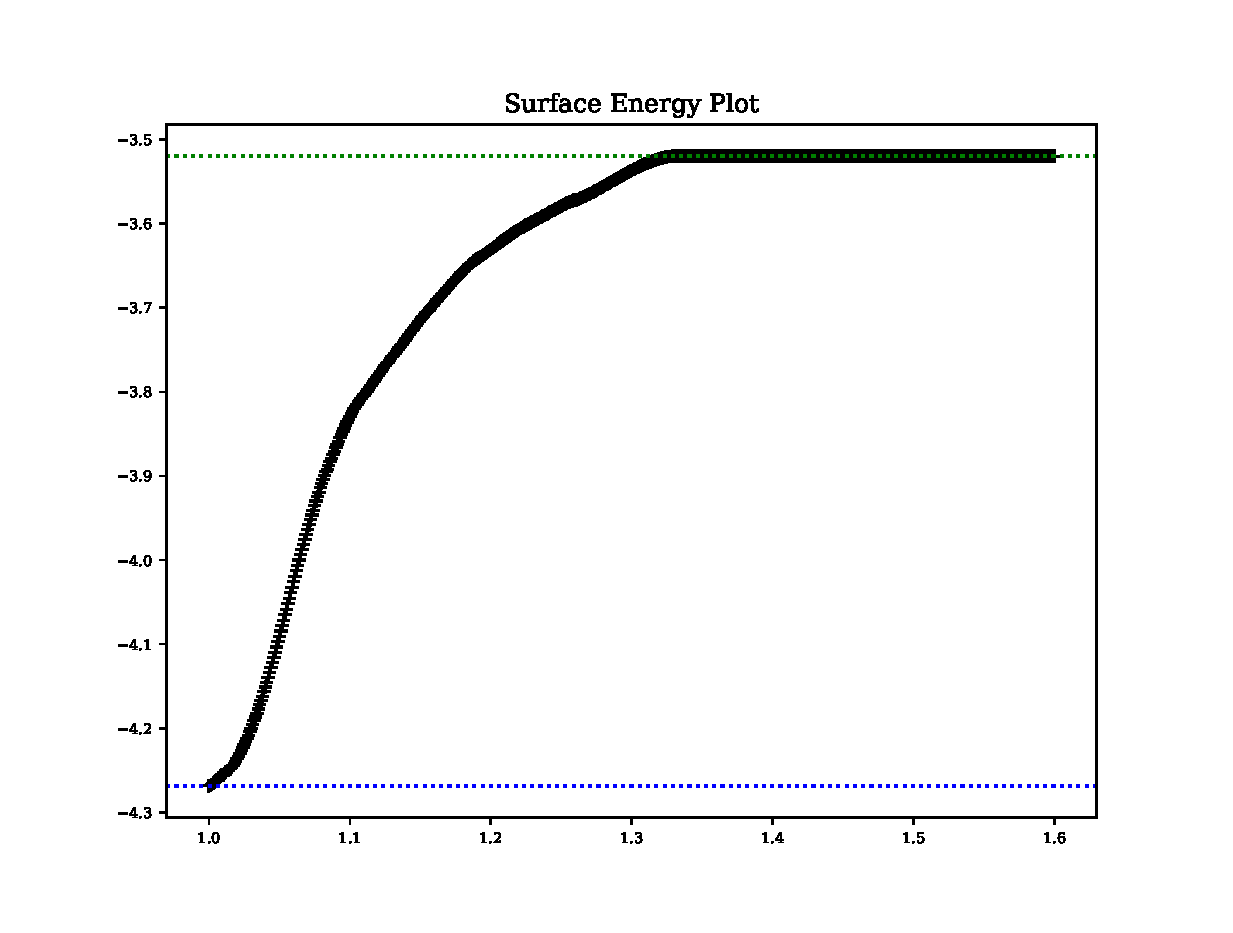
\includegraphics[width=.98\linewidth]{chapters/potentials_fe_pd_ru/pot_fepd_fcc_2/fe_surface_energy.eps} 
  \end{minipage}%%
  \begin{minipage}[b]{0.4\linewidth}
    \centering
    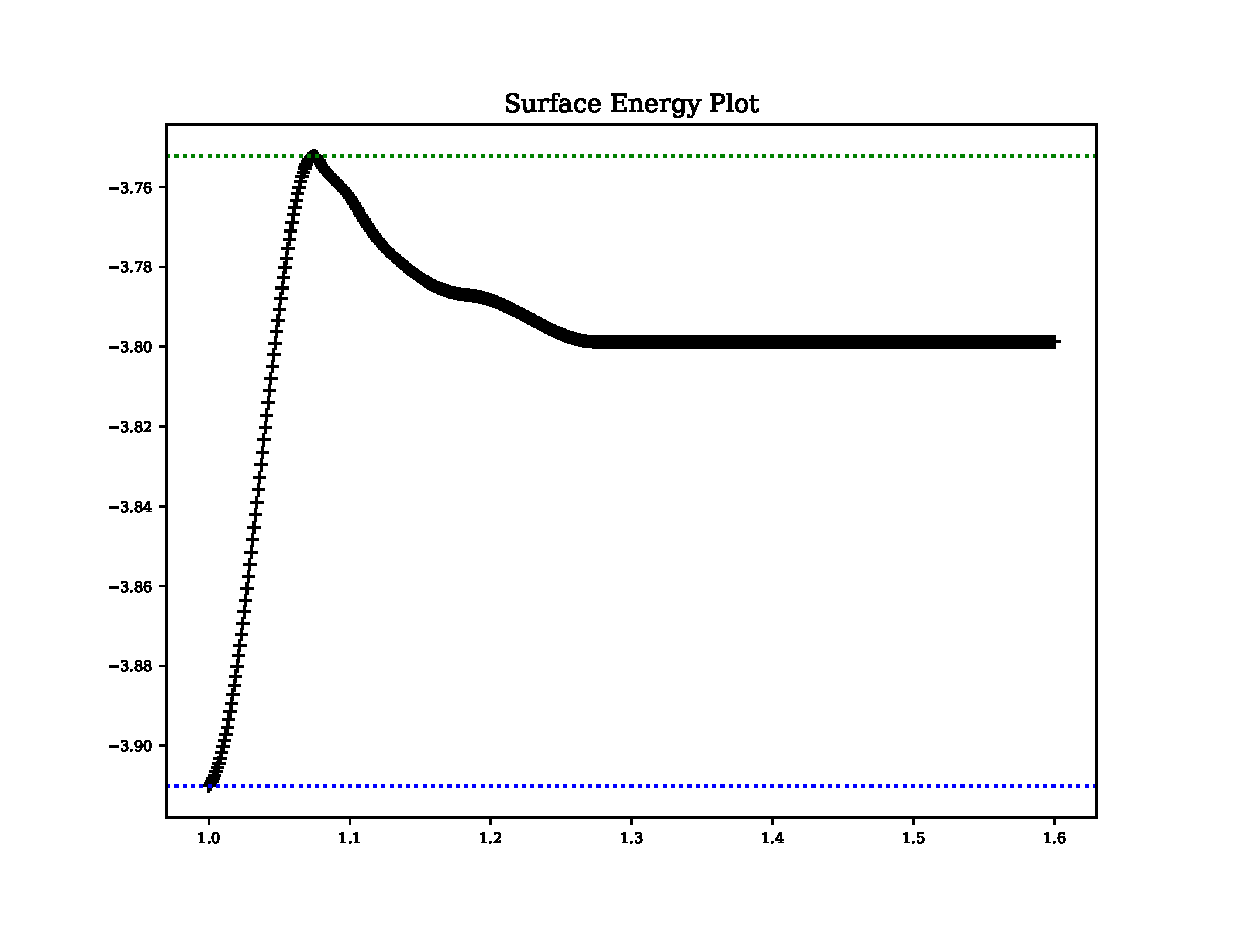
\includegraphics[width=.98\linewidth]{chapters/potentials_fe_pd_ru/pot_fepd_fcc_2/pd_surface_energy.eps} 
  \end{minipage}%%
	\caption{Cohesive energy and surface energy plots - detailed plots in the appendix \ref{fepdv2coh} and \ref{fepdv2se}}  
\label{fig:v2plots}
\end{figure}
\FloatBarrier

The non-cubic geometry of antiferromagnetic \acrshort{fcc} Fe also suggests that the energy surface should be considered in all three planes, both with \acrshort{dft} and in the fitting process.



\subsection{Original Contribution}

The fitting code is an original contribution as it allows the fitting of metal potentials in the form of the \acrlong{eam} and \acrlong{2beam} to \acrshort{dft} data and bulk properties.  Other similar codes do exist, such as FitPot and PotFit, but at the time of developing my code the PotFit did not have the ability to fit analytic potentials (although, this feature is now available) and does not have, in its available form, the ability to fit the potential to the bulk properties of the material (although the Sheng version did have this ability).  The code developed here may be modified in the future to add surface energy and point defect energies as data to fit to.  It would require the addition of a geometry relaxation subroutine to optimise the atom locations as the basis vectors change. 



\section{Two-Band EAM Contribution to DL-Poly}

During the early stages of this work it was clear that the Embedded Atom Method was a good candidate for the type of potential to be derived as it was well suited to modelling metals and had been used previously (along with the similar \acrshort{fs} potential) to model radiation damage\cite{damagebcciron}.  Work by Prof. Ackland at the University of Edinburgh considered using a separate density function and embedding functional to represent the S-Band and D-Band of transition elements such as Caesium.  Work by P. Olsson and J. Wallenius also used this two band version to model Fe-Cr with a later Fe-Cr potential being developed by Bonny et al to replicate the mixing enthalpy as a function of Cr content.  

After meeting with Prof. Todorov at Daresbury Laboratory, the source code for DL-Poly was modified to include new keywords, additional arrays to store the two-band density and embedding data for the second band and modifications to the energy and force subroutines.  This was then released with version 4.05 of DL\_POLY in July 2013.  

Ultimately, only \acrshort{eam} potentials were fit in this work.  In the future, as more elements are added to the potential, in particular Cr, the \acrshort{2beam} may be required.  The molecular dynamics code and fitting code both have the capability to use this type of potential.







